% Options for packages loaded elsewhere
\PassOptionsToPackage{unicode}{hyperref}
\PassOptionsToPackage{hyphens}{url}
\PassOptionsToPackage{dvipsnames,svgnames,x11names}{xcolor}
%
\documentclass[
  letterpaper,
  DIV=11,
  numbers=noendperiod]{scrreport}

\usepackage{amsmath,amssymb}
\usepackage{iftex}
\ifPDFTeX
  \usepackage[T1]{fontenc}
  \usepackage[utf8]{inputenc}
  \usepackage{textcomp} % provide euro and other symbols
\else % if luatex or xetex
  \usepackage{unicode-math}
  \defaultfontfeatures{Scale=MatchLowercase}
  \defaultfontfeatures[\rmfamily]{Ligatures=TeX,Scale=1}
\fi
\usepackage{lmodern}
\ifPDFTeX\else  
    % xetex/luatex font selection
\fi
% Use upquote if available, for straight quotes in verbatim environments
\IfFileExists{upquote.sty}{\usepackage{upquote}}{}
\IfFileExists{microtype.sty}{% use microtype if available
  \usepackage[]{microtype}
  \UseMicrotypeSet[protrusion]{basicmath} % disable protrusion for tt fonts
}{}
\makeatletter
\@ifundefined{KOMAClassName}{% if non-KOMA class
  \IfFileExists{parskip.sty}{%
    \usepackage{parskip}
  }{% else
    \setlength{\parindent}{0pt}
    \setlength{\parskip}{6pt plus 2pt minus 1pt}}
}{% if KOMA class
  \KOMAoptions{parskip=half}}
\makeatother
\usepackage{xcolor}
\setlength{\emergencystretch}{3em} % prevent overfull lines
\setcounter{secnumdepth}{5}
% Make \paragraph and \subparagraph free-standing
\ifx\paragraph\undefined\else
  \let\oldparagraph\paragraph
  \renewcommand{\paragraph}[1]{\oldparagraph{#1}\mbox{}}
\fi
\ifx\subparagraph\undefined\else
  \let\oldsubparagraph\subparagraph
  \renewcommand{\subparagraph}[1]{\oldsubparagraph{#1}\mbox{}}
\fi

\usepackage{color}
\usepackage{fancyvrb}
\newcommand{\VerbBar}{|}
\newcommand{\VERB}{\Verb[commandchars=\\\{\}]}
\DefineVerbatimEnvironment{Highlighting}{Verbatim}{commandchars=\\\{\}}
% Add ',fontsize=\small' for more characters per line
\usepackage{framed}
\definecolor{shadecolor}{RGB}{241,243,245}
\newenvironment{Shaded}{\begin{snugshade}}{\end{snugshade}}
\newcommand{\AlertTok}[1]{\textcolor[rgb]{0.68,0.00,0.00}{#1}}
\newcommand{\AnnotationTok}[1]{\textcolor[rgb]{0.37,0.37,0.37}{#1}}
\newcommand{\AttributeTok}[1]{\textcolor[rgb]{0.40,0.45,0.13}{#1}}
\newcommand{\BaseNTok}[1]{\textcolor[rgb]{0.68,0.00,0.00}{#1}}
\newcommand{\BuiltInTok}[1]{\textcolor[rgb]{0.00,0.23,0.31}{#1}}
\newcommand{\CharTok}[1]{\textcolor[rgb]{0.13,0.47,0.30}{#1}}
\newcommand{\CommentTok}[1]{\textcolor[rgb]{0.37,0.37,0.37}{#1}}
\newcommand{\CommentVarTok}[1]{\textcolor[rgb]{0.37,0.37,0.37}{\textit{#1}}}
\newcommand{\ConstantTok}[1]{\textcolor[rgb]{0.56,0.35,0.01}{#1}}
\newcommand{\ControlFlowTok}[1]{\textcolor[rgb]{0.00,0.23,0.31}{\textbf{#1}}}
\newcommand{\DataTypeTok}[1]{\textcolor[rgb]{0.68,0.00,0.00}{#1}}
\newcommand{\DecValTok}[1]{\textcolor[rgb]{0.68,0.00,0.00}{#1}}
\newcommand{\DocumentationTok}[1]{\textcolor[rgb]{0.37,0.37,0.37}{\textit{#1}}}
\newcommand{\ErrorTok}[1]{\textcolor[rgb]{0.68,0.00,0.00}{#1}}
\newcommand{\ExtensionTok}[1]{\textcolor[rgb]{0.00,0.23,0.31}{#1}}
\newcommand{\FloatTok}[1]{\textcolor[rgb]{0.68,0.00,0.00}{#1}}
\newcommand{\FunctionTok}[1]{\textcolor[rgb]{0.28,0.35,0.67}{#1}}
\newcommand{\ImportTok}[1]{\textcolor[rgb]{0.00,0.46,0.62}{#1}}
\newcommand{\InformationTok}[1]{\textcolor[rgb]{0.37,0.37,0.37}{#1}}
\newcommand{\KeywordTok}[1]{\textcolor[rgb]{0.00,0.23,0.31}{\textbf{#1}}}
\newcommand{\NormalTok}[1]{\textcolor[rgb]{0.00,0.23,0.31}{#1}}
\newcommand{\OperatorTok}[1]{\textcolor[rgb]{0.37,0.37,0.37}{#1}}
\newcommand{\OtherTok}[1]{\textcolor[rgb]{0.00,0.23,0.31}{#1}}
\newcommand{\PreprocessorTok}[1]{\textcolor[rgb]{0.68,0.00,0.00}{#1}}
\newcommand{\RegionMarkerTok}[1]{\textcolor[rgb]{0.00,0.23,0.31}{#1}}
\newcommand{\SpecialCharTok}[1]{\textcolor[rgb]{0.37,0.37,0.37}{#1}}
\newcommand{\SpecialStringTok}[1]{\textcolor[rgb]{0.13,0.47,0.30}{#1}}
\newcommand{\StringTok}[1]{\textcolor[rgb]{0.13,0.47,0.30}{#1}}
\newcommand{\VariableTok}[1]{\textcolor[rgb]{0.07,0.07,0.07}{#1}}
\newcommand{\VerbatimStringTok}[1]{\textcolor[rgb]{0.13,0.47,0.30}{#1}}
\newcommand{\WarningTok}[1]{\textcolor[rgb]{0.37,0.37,0.37}{\textit{#1}}}

\providecommand{\tightlist}{%
  \setlength{\itemsep}{0pt}\setlength{\parskip}{0pt}}\usepackage{longtable,booktabs,array}
\usepackage{calc} % for calculating minipage widths
% Correct order of tables after \paragraph or \subparagraph
\usepackage{etoolbox}
\makeatletter
\patchcmd\longtable{\par}{\if@noskipsec\mbox{}\fi\par}{}{}
\makeatother
% Allow footnotes in longtable head/foot
\IfFileExists{footnotehyper.sty}{\usepackage{footnotehyper}}{\usepackage{footnote}}
\makesavenoteenv{longtable}
\usepackage{graphicx}
\makeatletter
\def\maxwidth{\ifdim\Gin@nat@width>\linewidth\linewidth\else\Gin@nat@width\fi}
\def\maxheight{\ifdim\Gin@nat@height>\textheight\textheight\else\Gin@nat@height\fi}
\makeatother
% Scale images if necessary, so that they will not overflow the page
% margins by default, and it is still possible to overwrite the defaults
% using explicit options in \includegraphics[width, height, ...]{}
\setkeys{Gin}{width=\maxwidth,height=\maxheight,keepaspectratio}
% Set default figure placement to htbp
\makeatletter
\def\fps@figure{htbp}
\makeatother

\KOMAoption{captions}{tableheading}
\makeatletter
\@ifpackageloaded{bookmark}{}{\usepackage{bookmark}}
\makeatother
\makeatletter
\@ifpackageloaded{caption}{}{\usepackage{caption}}
\AtBeginDocument{%
\ifdefined\contentsname
  \renewcommand*\contentsname{Table of contents}
\else
  \newcommand\contentsname{Table of contents}
\fi
\ifdefined\listfigurename
  \renewcommand*\listfigurename{List of Figures}
\else
  \newcommand\listfigurename{List of Figures}
\fi
\ifdefined\listtablename
  \renewcommand*\listtablename{List of Tables}
\else
  \newcommand\listtablename{List of Tables}
\fi
\ifdefined\figurename
  \renewcommand*\figurename{Figure}
\else
  \newcommand\figurename{Figure}
\fi
\ifdefined\tablename
  \renewcommand*\tablename{Table}
\else
  \newcommand\tablename{Table}
\fi
}
\@ifpackageloaded{float}{}{\usepackage{float}}
\floatstyle{ruled}
\@ifundefined{c@chapter}{\newfloat{codelisting}{h}{lop}}{\newfloat{codelisting}{h}{lop}[chapter]}
\floatname{codelisting}{Listing}
\newcommand*\listoflistings{\listof{codelisting}{List of Listings}}
\makeatother
\makeatletter
\makeatother
\makeatletter
\@ifpackageloaded{caption}{}{\usepackage{caption}}
\@ifpackageloaded{subcaption}{}{\usepackage{subcaption}}
\makeatother
\ifLuaTeX
  \usepackage{selnolig}  % disable illegal ligatures
\fi
\usepackage{bookmark}

\IfFileExists{xurl.sty}{\usepackage{xurl}}{} % add URL line breaks if available
\urlstyle{same} % disable monospaced font for URLs
\hypersetup{
  pdfauthor={Pengfei Song},
  colorlinks=true,
  linkcolor={blue},
  filecolor={Maroon},
  citecolor={Blue},
  urlcolor={Blue},
  pdfcreator={LaTeX via pandoc}}

\author{Pengfei Song}
\date{2024-02-06}

\begin{document}

\renewcommand*\contentsname{Table of contents}
{
\hypersetup{linkcolor=}
\setcounter{tocdepth}{2}
\tableofcontents
}
\bookmarksetup{startatroot}

\chapter*{Welcome}\label{welcome}
\addcontentsline{toc}{chapter}{Welcome}

\markboth{Welcome}{Welcome}

\bookmarksetup{startatroot}

\chapter{Julia Basics}\label{julia-basics}

\section{Why Julia?}\label{why-julia}

Slow language is not suitable for this task --- learning neural networks
embedded in differential equations.

In short - Solving two language problems: \texttt{C++} is fast but
difficult; \texttt{Python} is easy but slow. \texttt{Julia} is fast and
easy. - Language for Mathematics: writing \texttt{Julia} is just like
writing mathematics. - Similar syntax as \texttt{Matlab}; Simple as
\texttt{Python}; Fast as \texttt{C++}.

More advantages and disadvantages can be seen in
\href{https://juliateachingctu.github.io/Julia-for-Optimization-and-Learning/stable/why/}{Why
Julia? · Julia for Optimization and Learning}

\section{Installation: Julia+VSCode}\label{installation-juliavscode}

\texttt{Julia} + \texttt{VScode}

\subsection{Recommended}\label{recommended}

We recommend to install Julia via
\href{https://github.com/JuliaLang/juliaup}{\texttt{juliaup}}. We are
using the latest, \emph{stable} version of Julia (which at the time of
this writing is \texttt{v1.10}). Once you have installed
\texttt{juliaup} you can get any Julia version you want via:

\begin{Shaded}
\begin{Highlighting}[]
\ExtensionTok{juliaup}\NormalTok{ add }\VariableTok{$JULIA\_VERSION}

\CommentTok{\# or more concretely:}
\ExtensionTok{juliaup}\NormalTok{ add 1.10}

\CommentTok{\# but please, just use the latest, stable version}
\end{Highlighting}
\end{Shaded}

Now you should be able to start Julia and be greeted with the following:

\begin{Shaded}
\begin{Highlighting}[]
\ExtensionTok{$}\NormalTok{ julia}
               \ExtensionTok{\_}
   \ExtensionTok{\_}\NormalTok{       \_ \_}\ErrorTok{(}\ExtensionTok{\_}\KeywordTok{)}\ExtensionTok{\_}     \KeywordTok{|}  \ExtensionTok{Documentation:}\NormalTok{ https://docs.julialang.org}
  \KeywordTok{(}\ExtensionTok{\_}\KeywordTok{)}     \KeywordTok{|} \KeywordTok{(}\ExtensionTok{\_}\KeywordTok{)} \KeywordTok{(}\ExtensionTok{\_}\KeywordTok{)}    \KeywordTok{|}
   \ExtensionTok{\_}\NormalTok{ \_   \_}\KeywordTok{|} \KeywordTok{|}\ExtensionTok{\_}\NormalTok{  \_\_ \_   }\KeywordTok{|}  \ExtensionTok{Type} \StringTok{"?"}\NormalTok{ for help, }\StringTok{"]?"}\NormalTok{ for Pkg help.}
  \KeywordTok{|} \KeywordTok{|} \KeywordTok{|} \KeywordTok{|} \KeywordTok{|} \KeywordTok{|} \KeywordTok{|}\ExtensionTok{/}\NormalTok{ \_}\KeywordTok{\textasciigrave{}} \KeywordTok{|}  \KeywordTok{|}
  \KeywordTok{|} \KeywordTok{|} \KeywordTok{|}\ExtensionTok{\_}\KeywordTok{|} \KeywordTok{|} \KeywordTok{|} \KeywordTok{|} \KeywordTok{(}\ExtensionTok{\_}\KeywordTok{|} \KeywordTok{|}  \KeywordTok{|}  \ExtensionTok{Version}\NormalTok{ 1.10.0 }\ErrorTok{(}\ExtensionTok{2023{-}12{-}25}\KeywordTok{)}
 \ExtensionTok{\_/} \KeywordTok{|}\ExtensionTok{\textbackslash{}\_\_}\StringTok{\textquotesingle{}\_|\_|\_|\textbackslash{}\_\_\textquotesingle{}}\ExtensionTok{\_}\KeywordTok{|}  \KeywordTok{|}  \ExtensionTok{Official}\NormalTok{ https://julialang.org/ release}
\KeywordTok{|}\ExtensionTok{\_\_/}                   \KeywordTok{|}

\ExtensionTok{julia}\OperatorTok{\textgreater{}}
\end{Highlighting}
\end{Shaded}

\subsection{Alternatives}\label{alternatives}

Julia can also be installed from the official website
\href{https://julialang.org/downloads/}{download page}. The appropriate
version is the \textbf{64-bits} version for the Windows operating system
in most cases. In case of difficulties, see
\href{https://julialang.org/downloads/platform/}{platform-specific
instructions}.

\subsection{Editor}\label{editor}

There is no one way to install/develop and run Julia, which may be
strange for users coming from MATLAB, but for users of general purpose
languages such as Python, C++ this is quite common. Most of the Julia
programmers to date are using

\begin{itemize}
\tightlist
\item
  \href{https://code.visualstudio.com/}{Visual Studio Code},
\item
  and the corresponding \href{https://www.julia-vscode.org/}{Julia
  extension}.
\end{itemize}

This setup is described in a comprehensive
\href{https://juliateachingctu.github.io/Julia-for-Optimization-and\%20Learning/stable/installation/vscode/}{step-by-step
guide} in
\href{https://juliateachingctu.github.io/Julia-for-Optimization-and-Learning/stable/}{\emph{Julia
for Optimization \& Learning}}.

For other editors, we refer to \href{https://julialang.org/}{Julia IDE}

\section{Packages and Environment
Management}\label{packages-and-environment-management}

\texttt{Julia} manages packages and environments like \texttt{Rust}.
Very convenient! Strongly recommendation: go through this document
\href{https://pkgdocs.julialang.org/v1/environments/\#Working-with-Environments}{Working
with Environment · Pkg.jl} quickly.

To set up the same environment as me, you can follow the guides in
\href{https://github.com/Song921012/Julia_Tutorial_on_AI4MathBiology}{Song921012/Julia\_Tutorial\_on\_AI4MathBiology}

\section{Other Julia Courses and
Materials}\label{other-julia-courses-and-materials}

\begin{itemize}
\tightlist
\item
  \href{https://docs.julialang.org/en/v1/}{Official documentation}
\item
  Slack channel: \href{https://julialang.org/community/}{Community}
\item
  Important:\href{https://cheatsheets.quantecon.org/}{Cheatsheet for
  differences between Julia and Matlab and Python}
\item
  \href{https://cheatsheets.quantecon.org/julia-cheatsheet.html}{Cheatsheet
  of basic functions}
\item
  \href{https://juliadocs.github.io/Julia-Cheat-Sheet/}{Cheatsheet of
  advanced functions}
\item
  \href{https://benlauwens.github.io/ThinkJulia.jl/latest/book.html\#chap01}{Think
  Julia: How to Think Like a Computer Scientist}
\item
  \href{https://techytok.com/from-zero-to-julia/}{From Zero to Julia!}
\item
  Recommended:
  \href{https://juliateachingctu.github.io/Julia-for-Optimization-and-Learning/stable/}{Julia
  for Optimization and Learning}
\item
  \href{https://juliateachingctu.github.io/Scientific-Programming-in-Julia/dev/}{Scientific
  Programming in Julia}
\item
  \href{https://juliadatascience.io/}{Julia Data Science}
\item
  \href{https://statisticswithjulia.org/}{Statistics with Julia:
  Fundamentals for Data Science, Machine Learning and Artificial
  Intelligence}
\end{itemize}

\bookmarksetup{startatroot}

\chapter{Neural Networks}\label{neural-networks}

Neural network is no mystery, it is just a function with powerful
learning ability.

At this time, you don't need to care much details about its complicated
structure.

In Julia, two deep learning packages are commonly used: -
\texttt{Flux.jl}:\href{https://fluxml.ai/Flux.jl/stable/}{Welcome ·
Flux} - \texttt{Lux.jl}:\href{https://lux.csail.mit.edu/}{LuxDL Docs}

Here, we use \texttt{Flux.jl} as an example. More details can be seen in
packages official documents.

\section{IMPORTANT: Activate Julia environment
first}\label{important-activate-julia-environment-first}

\begin{Shaded}
\begin{Highlighting}[]
\ImportTok{using} \BuiltInTok{Pkg}
\BuiltInTok{Pkg}\NormalTok{.}\FunctionTok{activate}\NormalTok{(}\StringTok{"."}\NormalTok{)}
\end{Highlighting}
\end{Shaded}

\begin{verbatim}
  Activating project at `~/Desktop/MyProjects/Julia_Tutorial_on_AI4MathBiology`
\end{verbatim}

\section{Multilayer neural network as a
function}\label{multilayer-neural-network-as-a-function}

You only need to regard neural network as a function \(f(x,p)\), \(x\)
input, \(p\) parameters.

\begin{Shaded}
\begin{Highlighting}[]
\ImportTok{using} \BuiltInTok{Flux}
\NormalTok{dnn\_model }\OperatorTok{=} \FunctionTok{Chain}\NormalTok{(}\FunctionTok{Dense}\NormalTok{(}\FloatTok{1}\NormalTok{, }\FloatTok{10}\NormalTok{, swish), }\FunctionTok{Dense}\NormalTok{(}\FloatTok{10}\NormalTok{, }\FloatTok{100}\NormalTok{,swish),}\FunctionTok{Dense}\NormalTok{(}\FloatTok{100}\NormalTok{, }\FloatTok{10}\NormalTok{, swish), }\FunctionTok{Dense}\NormalTok{(}\FloatTok{10}\NormalTok{, }\FloatTok{1}\NormalTok{))}
\CommentTok{\# Remark: In Deep Learning, there is no one dimensional scalar but one dimensional vector }
\FunctionTok{dnn\_model}\NormalTok{([}\FloatTok{1.0f0}\NormalTok{])}
\end{Highlighting}
\end{Shaded}

\begin{verbatim}
1-element Vector{Float32}:
 -0.040261105
\end{verbatim}

\begin{Shaded}
\begin{Highlighting}[]
\NormalTok{dnn\_model2 }\OperatorTok{=} \FunctionTok{Chain}\NormalTok{(}\FunctionTok{Dense}\NormalTok{(}\FloatTok{2}\NormalTok{, }\FloatTok{10}\NormalTok{, swish), }\FunctionTok{Dense}\NormalTok{(}\FloatTok{10}\NormalTok{, }\FloatTok{100}\NormalTok{,swish),}\FunctionTok{Dense}\NormalTok{(}\FloatTok{100}\NormalTok{, }\FloatTok{10}\NormalTok{, swish), }\FunctionTok{Dense}\NormalTok{(}\FloatTok{10}\NormalTok{, }\FloatTok{2}\NormalTok{))}
\CommentTok{\# Remark: f0 here means we use Float32}
\FunctionTok{dnn\_model2}\NormalTok{([}\FloatTok{1.0f0}\NormalTok{,}\FloatTok{2.0f0}\NormalTok{])[}\FloatTok{1}\NormalTok{]}
\end{Highlighting}
\end{Shaded}

\begin{verbatim}
0.100376524f0
\end{verbatim}

Note here that we didn't set parameters for this deep learning
architecture, however, it has an input. Why?

The reason is that in \texttt{Flux.jl}, a DNN model has parameters pre
defined. Sometimes, it is very inconvenient. Thus, we need to
destructure the neural network, so that we can change the parameter of
the neural network.

\section{IMPORTANT: destructure}\label{important-destructure}

\begin{Shaded}
\begin{Highlighting}[]
\NormalTok{parameter, structure}\OperatorTok{=}\NormalTok{Flux.}\FunctionTok{destructure}\NormalTok{(dnn\_model2) }\CommentTok{\# parameters and structures}
\NormalTok{newpara }\OperatorTok{=}\NormalTok{ parameter}\OperatorTok{*}\FloatTok{0.1} \OperatorTok{.+} \FloatTok{0.3}
\CommentTok{\# DNN with new parameters}
\FunctionTok{f}\NormalTok{(x,p)}\OperatorTok{=}\FunctionTok{structure}\NormalTok{(p)(x)}\CommentTok{\# x input, p parameter}
\FunctionTok{println}\NormalTok{(}\StringTok{"DNN with new parameter:"}\NormalTok{, }\FunctionTok{f}\NormalTok{([}\FloatTok{1.0f0}\NormalTok{,}\FloatTok{2.0f0}\NormalTok{],newpara))}
\end{Highlighting}
\end{Shaded}

\begin{verbatim}
DNN with new parameter:Float32[286.11746, 278.07166]
\end{verbatim}

\section{\texorpdfstring{Using DNN to learn
\(\sin(x)\)}{Using DNN to learn \textbackslash sin(x)}}\label{using-dnn-to-learn-sinx}

\begin{Shaded}
\begin{Highlighting}[]
\ImportTok{using} \BuiltInTok{Flux}
\ImportTok{using} \BuiltInTok{Flux}\NormalTok{:train!,params}
\CommentTok{\# 1. Gennerate Data and Define DNN}
\NormalTok{x }\OperatorTok{=} \FunctionTok{Array}\NormalTok{(}\OperatorTok{{-}}\FloatTok{2}\NormalTok{π}\OperatorTok{:}\FloatTok{0.01}\OperatorTok{:}\FloatTok{2}\NormalTok{π)}\CharTok{\textquotesingle{}}
\NormalTok{data }\OperatorTok{=} \FunctionTok{sin}\NormalTok{.(x)}
\CommentTok{\#dnn\_model = Chain(Dense(1, 1), x{-}\textgreater{} cos.(x))}
\CommentTok{\#dnn\_model = Chain(Dense(1, 128, relu), Dense(128, 1), x{-}\textgreater{} cos.(x))}
\NormalTok{dnn\_model }\OperatorTok{=} \FunctionTok{Chain}\NormalTok{(}\FunctionTok{Dense}\NormalTok{(}\FloatTok{1}\NormalTok{, }\FloatTok{10}\NormalTok{, swish), }\FunctionTok{Dense}\NormalTok{(}\FloatTok{10}\NormalTok{, }\FloatTok{100}\NormalTok{,swish),}\FunctionTok{Dense}\NormalTok{(}\FloatTok{100}\NormalTok{, }\FloatTok{10}\NormalTok{, swish), }\FunctionTok{Dense}\NormalTok{(}\FloatTok{10}\NormalTok{, }\FloatTok{1}\NormalTok{))}
\CommentTok{\# dnn\_model = Chain(Dense(1, 32, relu), Dense(32, 1, tanh))}


\CommentTok{\# 2. Define Loss Functions}
\FunctionTok{loss2}\NormalTok{(a,b) }\OperatorTok{=}\NormalTok{ Flux.Losses.}\FunctionTok{mae}\NormalTok{(}\FunctionTok{dnn\_model}\NormalTok{(x), data)}

\CommentTok{\# Train the model}
\NormalTok{opt}\OperatorTok{=}\FunctionTok{ADAM}\NormalTok{(}\FloatTok{0.02}\NormalTok{)}
\FunctionTok{println}\NormalTok{(}\FunctionTok{loss2}\NormalTok{(x, data))}
\FunctionTok{train!}\NormalTok{(loss2, Flux.}\FunctionTok{params}\NormalTok{(dnn\_model), [(x,data)], opt)}
\FunctionTok{println}\NormalTok{(}\FunctionTok{loss2}\NormalTok{(x, data))}



\ControlFlowTok{for}\NormalTok{ epoch }\KeywordTok{in} \FloatTok{1}\OperatorTok{:}\FloatTok{5000}
    \FunctionTok{train!}\NormalTok{(loss2, }\FunctionTok{params}\NormalTok{(dnn\_model), [(x,data)], opt)}
    \ControlFlowTok{if}\NormalTok{ epoch}\OperatorTok{\%}\FloatTok{500}\OperatorTok{==}\FloatTok{0}
    \FunctionTok{println}\NormalTok{(}\FunctionTok{loss2}\NormalTok{(x, data))}
    \ControlFlowTok{end}
\ControlFlowTok{end}
\end{Highlighting}
\end{Shaded}

\begin{verbatim}
0.6178579239993328
0.8133888838007648
0.029455694189493377
0.019722234455541977
0.02941249289718608
0.044564484807402126
0.017978833994311296
0.018942334715419555
0.04541769339893456
0.019092272589503845
0.020229457337176477
0.02070247009650008
\end{verbatim}

Data visulization

\begin{Shaded}
\begin{Highlighting}[]
\ImportTok{using} \BuiltInTok{Plots}
\FunctionTok{println}\NormalTok{(}\FunctionTok{loss2}\NormalTok{(x, data))}
\NormalTok{y }\OperatorTok{=} \FunctionTok{Array}\NormalTok{(}\OperatorTok{{-}}\FloatTok{2}\NormalTok{π}\OperatorTok{:}\FloatTok{0.1}\OperatorTok{:}\FloatTok{4}\NormalTok{π)}\CharTok{\textquotesingle{}}
\FunctionTok{scatter}\NormalTok{(}\FunctionTok{sin}\NormalTok{.(y)}\CharTok{\textquotesingle{})}
\FunctionTok{plot!}\NormalTok{(}\FunctionTok{dnn\_model}\NormalTok{(y)}\CharTok{\textquotesingle{})}
\end{Highlighting}
\end{Shaded}

\begin{verbatim}
0.02070247009650008
\end{verbatim}

\includegraphics{index_files/mediabag/2-neural-networks&optimization_files/figure-pdf/cell-7-output-2.pdf}

\subsection{\texorpdfstring{Question: why this DNN learn the \(\sin(x)\)
data but fails to predict \(\sin(x)\)? How to improve the
performance?}{Question: why this DNN learn the \textbackslash sin(x) data but fails to predict \textbackslash sin(x)? How to improve the performance?}}\label{question-why-this-dnn-learn-the-sinx-data-but-fails-to-predict-sinx-how-to-improve-the-performance}

\section{Optimization}\label{optimization}

Training a deep learning model is an optimization problem. In Julia,
there is a unified optimization package with many popular optimizers,
such as LBFS, BFGS, ADAM, SGD, evolution algorithms. For more details,
one can seen -
\href{https://docs.sciml.ai/Optimization/stable/}{Optimization.jl: A
Unified Optimization Package · Optimization.jl}

At this time, you only need to understand the following example:
\[\min_{x} (x_1-p_1)^2+p_2*(x_2-x_1^2)^2\] where \(p\) is parameter you
can pre defined.

\begin{Shaded}
\begin{Highlighting}[]
\CommentTok{\# Import the package and define the problem to optimize}
\ImportTok{using} \BuiltInTok{Optimization}
\FunctionTok{rosenbrock}\NormalTok{(u, p) }\OperatorTok{=}\NormalTok{ (p[}\FloatTok{1}\NormalTok{] }\OperatorTok{{-}}\NormalTok{ u[}\FloatTok{1}\NormalTok{])}\OperatorTok{\^{}}\FloatTok{2} \OperatorTok{+}\NormalTok{ p[}\FloatTok{2}\NormalTok{] }\OperatorTok{*}\NormalTok{ (u[}\FloatTok{2}\NormalTok{] }\OperatorTok{{-}}\NormalTok{ u[}\FloatTok{1}\NormalTok{]}\OperatorTok{\^{}}\FloatTok{2}\NormalTok{)}\OperatorTok{\^{}}\FloatTok{2}
\NormalTok{u0 }\OperatorTok{=} \FunctionTok{zeros}\NormalTok{(}\FloatTok{2}\NormalTok{)}
\NormalTok{p }\OperatorTok{=}\NormalTok{ [}\FloatTok{1.0}\NormalTok{, }\FloatTok{100.0}\NormalTok{]}

\NormalTok{prob }\OperatorTok{=} \FunctionTok{OptimizationProblem}\NormalTok{(rosenbrock, u0, p)}

\CommentTok{\# Import a solver package and solve the optimization problem}
\ImportTok{using} \BuiltInTok{OptimizationOptimJL}
\NormalTok{sol }\OperatorTok{=} \FunctionTok{solve}\NormalTok{(prob, }\FunctionTok{NelderMead}\NormalTok{())}
\end{Highlighting}
\end{Shaded}

\begin{verbatim}
retcode: Success
u: 2-element Vector{Float64}:
 0.9999634355313174
 0.9999315506115275
\end{verbatim}

Import a different solver package and solve the optimization problem a
different way

\begin{Shaded}
\begin{Highlighting}[]
\ImportTok{using} \BuiltInTok{OptimizationBBO}
\NormalTok{prob }\OperatorTok{=} \FunctionTok{OptimizationProblem}\NormalTok{(rosenbrock, u0, p, lb }\OperatorTok{=}\NormalTok{ [}\OperatorTok{{-}}\FloatTok{1.0}\NormalTok{, }\OperatorTok{{-}}\FloatTok{1.0}\NormalTok{], ub }\OperatorTok{=}\NormalTok{ [}\FloatTok{1.0}\NormalTok{, }\FloatTok{1.0}\NormalTok{])}
\NormalTok{sol }\OperatorTok{=} \FunctionTok{solve}\NormalTok{(prob, }\FunctionTok{BBO\_adaptive\_de\_rand\_1\_bin\_radiuslimited}\NormalTok{())}
\end{Highlighting}
\end{Shaded}

\begin{verbatim}
retcode: Failure
u: 2-element Vector{Float64}:
 0.9999999999999876
 0.9999999999999785
\end{verbatim}

\bookmarksetup{startatroot}

\chapter{Differential Equations}\label{differential-equations}

\subsection{Solving SIR Model}\label{solving-sir-model}

More details can be seen in

\href{https://docs.sciml.ai/DiffEqDocs/stable/getting_started/}{Getting
Started with Differential Equations in Julia · DifferentialEquations.jl}

\href{https://github.com/SciML/DifferentialEquations.jl}{SciML/DifferentialEquations.jl:
Multi-language suite for high-performance solvers of differential
equations and scientific machine learning (SciML) components. Ordinary
differential equations (ODEs), stochastic differential equations (SDEs),
delay differential equations (DDEs), differential-algebraic equations
(DAEs), and more in Julia.}

\section{IMPORTANT: Activate Julia environment
first}\label{important-activate-julia-environment-first-1}

\begin{Shaded}
\begin{Highlighting}[]
\ImportTok{using} \BuiltInTok{Pkg}
\BuiltInTok{Pkg}\NormalTok{.}\FunctionTok{activate}\NormalTok{(}\StringTok{"."}\NormalTok{)}
\end{Highlighting}
\end{Shaded}

\begin{verbatim}
  Activating project at `~/Desktop/MyProjects/Julia_Tutorial_on_AI4MathBiology`
\end{verbatim}

\subsection{Learn Julia in AI era}\label{learn-julia-in-ai-era}

Actually, you can also use \href{https://cursor.sh/}{Cursor - The
AI-first Code Editor} (VSCode with ChatGPT embedded.)

\begin{Shaded}
\begin{Highlighting}[]
\ImportTok{using} \BuiltInTok{DifferentialEquations}
\KeywordTok{function} \FunctionTok{sir!}\NormalTok{(du,u,p,t)}
\NormalTok{    S,I,R }\OperatorTok{=}\NormalTok{ u}
\NormalTok{    β,γ }\OperatorTok{=}\NormalTok{ p}
\NormalTok{    du[}\FloatTok{1}\NormalTok{] }\OperatorTok{=} \OperatorTok{{-}}\NormalTok{β}\OperatorTok{*}\NormalTok{S}\OperatorTok{*}\NormalTok{I}
\NormalTok{    du[}\FloatTok{2}\NormalTok{] }\OperatorTok{=}\NormalTok{ β}\OperatorTok{*}\NormalTok{S}\OperatorTok{*}\NormalTok{I}\OperatorTok{{-}}\NormalTok{γ}\OperatorTok{*}\NormalTok{I}
\NormalTok{    du[}\FloatTok{3}\NormalTok{] }\OperatorTok{=}\NormalTok{ γ}\OperatorTok{*}\NormalTok{I}
\KeywordTok{end}
\NormalTok{parms }\OperatorTok{=}\NormalTok{ [}\FloatTok{0.1}\NormalTok{,}\FloatTok{0.05}\NormalTok{]}
\NormalTok{initialvalue }\OperatorTok{=}\NormalTok{ [}\FloatTok{0.99}\NormalTok{,}\FloatTok{0.01}\NormalTok{,}\FloatTok{0.0}\NormalTok{]}
\NormalTok{tspan }\OperatorTok{=}\NormalTok{ (}\FloatTok{0.0}\NormalTok{,}\FloatTok{200.0}\NormalTok{)}
\NormalTok{sir\_prob }\OperatorTok{=} \FunctionTok{ODEProblem}\NormalTok{(sir!,initialvalue,tspan,parms)}
\NormalTok{sir\_sol }\OperatorTok{=} \FunctionTok{solve}\NormalTok{(sir\_prob,saveat }\OperatorTok{=} \FloatTok{0.1}\NormalTok{);}
\end{Highlighting}
\end{Shaded}

\subsection{Data visulization}\label{data-visulization}

In Julia, we use \texttt{Plots.jl} or \texttt{Makie.jl} or
\texttt{TidierPlots.jl}(similar to \texttt{ggplot2})

\begin{itemize}
\item
  \href{https://docs.juliaplots.org/stable/}{Plots.jl}
\item
  \href{https://docs.makie.org/stable/}{Makie.jl}
\item
  \href{https://github.com/TidierOrg/TidierPlots.jl}{TidierOrg/TidierPlots.jl:
  Tidier data visualization in Julia, modeled after the ggplot2 R
  package.}
\end{itemize}

\begin{Shaded}
\begin{Highlighting}[]
\ImportTok{using} \BuiltInTok{Plots}
\FunctionTok{plot}\NormalTok{(sir\_sol)}
\end{Highlighting}
\end{Shaded}

\includegraphics{index_files/mediabag/3-differential-equations_files/figure-pdf/cell-4-output-1.pdf}

\section{Solving SIR model with neural networks
embedded}\label{solving-sir-model-with-neural-networks-embedded}

Solving the following differential equations with neural networks
embedded \[
    \left\{
    \begin{aligned}
         & \frac{\mathrm{d}S}{\mathrm{dt}} = - \mathrm{NN}(I) S ,        \\
         & \frac{\mathrm{d}I}{\mathrm{dt}} = \mathrm{NN}(I) S- \gamma I,
    \end{aligned}
    \right.
\]

\begin{Shaded}
\begin{Highlighting}[]
\ImportTok{using} \BuiltInTok{DifferentialEquations}
\ImportTok{using} \BuiltInTok{Flux}
\ImportTok{using} \BuiltInTok{Plots}
\NormalTok{ann\_node }\OperatorTok{=}\NormalTok{ Flux.}\FunctionTok{Chain}\NormalTok{(Flux.}\FunctionTok{Dense}\NormalTok{(}\FloatTok{1}\NormalTok{, }\FloatTok{64}\NormalTok{, tanh), Flux.}\FunctionTok{Dense}\NormalTok{(}\FloatTok{64}\NormalTok{, }\FloatTok{1}\NormalTok{))}
\NormalTok{para, re }\OperatorTok{=}\NormalTok{ Flux.}\FunctionTok{destructure}\NormalTok{(ann\_node) }\CommentTok{\# destructure}
\KeywordTok{function} \FunctionTok{SIR\_nn}\NormalTok{(du,u,p,t)}
\NormalTok{    S, I }\OperatorTok{=}\NormalTok{ u}
\NormalTok{    du[}\FloatTok{1}\NormalTok{] }\OperatorTok{=}  \OperatorTok{{-}} \FunctionTok{S*re}\NormalTok{(p)([I])[}\FloatTok{1}\NormalTok{]}
\NormalTok{    du[}\FloatTok{2}\NormalTok{] }\OperatorTok{=} \FunctionTok{S*re}\NormalTok{(p)([I])[}\FloatTok{1}\NormalTok{] }\OperatorTok{{-}} \FloatTok{0.1}\OperatorTok{*}\NormalTok{I}
\KeywordTok{end}
\NormalTok{initialvalue }\OperatorTok{=} \FunctionTok{Float32}\NormalTok{.([}\FloatTok{0.99}\NormalTok{,}\FloatTok{0.01}\NormalTok{])}
\NormalTok{tspan }\OperatorTok{=}\NormalTok{ (}\FloatTok{0.0f0}\NormalTok{,}\FloatTok{200.0f0}\NormalTok{)}
\NormalTok{prob\_nn }\OperatorTok{=} \FunctionTok{ODEProblem}\NormalTok{(SIR\_nn, initialvalue, tspan, para)}
\NormalTok{sol\_nn}\OperatorTok{=}\FunctionTok{solve}\NormalTok{(prob\_nn)}
\FunctionTok{plot}\NormalTok{(sol\_nn)}
\end{Highlighting}
\end{Shaded}

\includegraphics{index_files/mediabag/3-differential-equations_files/figure-pdf/cell-5-output-1.pdf}

\bookmarksetup{startatroot}

\chapter{Couple of differential equations and deep
learning}\label{couple-of-differential-equations-and-deep-learning}

Now we will apply UDE \[\left\{
\begin{aligned}
    & I' = \gamma \mathrm{NeuralNetwork}_{\theta}(t,I) I  -\gamma I,\\
    & \mathcal{R}_t = \mathrm{NeuralNetwork}_{\theta}(t,I),
\end{aligned}
\right.\] to learn effective reproduction number from the data generated
by logistic model \[
    \left\{
    \begin{aligned}
        & I' = 0.2\left(1-\frac{I}{30}\right)I,\\
        & \mathcal{R}_t = 3-\frac{I}{15}.
    \end{aligned}
    \right.
\]

For detail on mathematics, one can see - Song P, Xiao Y. Estimating
time-varying reproduction number by deep learning techniques{[}J{]}. J
Appl Anal Comput, 2022, 12(3): 1077-1089.

\section{IMPORTANT: Activate Julia environment
first}\label{important-activate-julia-environment-first-2}

\begin{Shaded}
\begin{Highlighting}[]
\ImportTok{using} \BuiltInTok{Pkg}
\BuiltInTok{Pkg}\NormalTok{.}\FunctionTok{activate}\NormalTok{(}\StringTok{"."}\NormalTok{)}
\end{Highlighting}
\end{Shaded}

\begin{verbatim}
  Activating project at `~/Desktop/MyProjects/Julia_Tutorial_on_AI4MathBiology`
\end{verbatim}

\section{Loading packages and setting random
seeds}\label{loading-packages-and-setting-random-seeds}

\begin{Shaded}
\begin{Highlighting}[]
\CommentTok{\#\#}
\ImportTok{using} \BuiltInTok{Lux}\NormalTok{, }\BuiltInTok{DiffEqFlux}\NormalTok{, }\BuiltInTok{DifferentialEquations}\NormalTok{, }\BuiltInTok{Optimization}\NormalTok{, }\BuiltInTok{OptimizationOptimJL}\NormalTok{, }\BuiltInTok{Random}\NormalTok{, }\BuiltInTok{Plots}
\ImportTok{using} \BuiltInTok{DataFrames}
\ImportTok{using} \BuiltInTok{CSV}
\ImportTok{using} \BuiltInTok{ComponentArrays}
\ImportTok{using} \BuiltInTok{OptimizationOptimisers}
\ImportTok{using} \BuiltInTok{Flux}
\ImportTok{using} \BuiltInTok{Plots}
\ImportTok{using} \BuiltInTok{LaTeXStrings}
\NormalTok{rng }\OperatorTok{=} \BuiltInTok{Random}\NormalTok{.}\FunctionTok{default\_rng}\NormalTok{()}
\BuiltInTok{Random}\NormalTok{.}\FunctionTok{seed!}\NormalTok{(}\FloatTok{1}\NormalTok{);}
\end{Highlighting}
\end{Shaded}

\section{Generating test data from logistic
model}\label{generating-test-data-from-logistic-model}

\begin{Shaded}
\begin{Highlighting}[]
\KeywordTok{function} \FunctionTok{model2}\NormalTok{(du, u, p, t)}
\NormalTok{    r, α }\OperatorTok{=}\NormalTok{ p}
\NormalTok{    du }\OperatorTok{.=}\NormalTok{ r }\OperatorTok{.*}\NormalTok{ u }\OperatorTok{.*}\NormalTok{ (}\FloatTok{1} \OperatorTok{.{-}}\NormalTok{ u }\OperatorTok{./}\NormalTok{ α)}
\KeywordTok{end}
\NormalTok{u\_0 }\OperatorTok{=}\NormalTok{ [}\FloatTok{1.0}\NormalTok{]}
\NormalTok{p\_data }\OperatorTok{=}\NormalTok{ [}\FloatTok{0.2}\NormalTok{, }\FloatTok{30}\NormalTok{]}
\NormalTok{tspan\_data }\OperatorTok{=}\NormalTok{ (}\FloatTok{0.0}\NormalTok{, }\FloatTok{30}\NormalTok{)}
\NormalTok{prob\_data }\OperatorTok{=} \FunctionTok{ODEProblem}\NormalTok{(model2, u\_0, tspan\_data, p\_data)}
\NormalTok{data\_solve }\OperatorTok{=} \FunctionTok{solve}\NormalTok{(prob\_data, }\FunctionTok{Tsit5}\NormalTok{(), abstol}\OperatorTok{=}\FloatTok{1e{-}12}\NormalTok{, reltol}\OperatorTok{=}\FloatTok{1e{-}12}\NormalTok{, saveat}\OperatorTok{=}\FloatTok{1}\NormalTok{)}
\NormalTok{data\_withoutnois }\OperatorTok{=} \FunctionTok{Array}\NormalTok{(data\_solve)}
\NormalTok{data }\OperatorTok{=}\NormalTok{ data\_withoutnois }\CommentTok{\#+ Float32(2e{-}1)*randn(eltype(data\_withoutnois), size(data\_withoutnois))}
\NormalTok{tspan\_predict }\OperatorTok{=}\NormalTok{ (}\FloatTok{0.0}\NormalTok{, }\FloatTok{40}\NormalTok{)}
\NormalTok{prob\_predict }\OperatorTok{=} \FunctionTok{ODEProblem}\NormalTok{(model2, u\_0, tspan\_predict, p\_data)}
\NormalTok{test\_data }\OperatorTok{=} \FunctionTok{solve}\NormalTok{(prob\_predict, }\FunctionTok{Tsit5}\NormalTok{(), abstol}\OperatorTok{=}\FloatTok{1e{-}12}\NormalTok{, reltol}\OperatorTok{=}\FloatTok{1e{-}12}\NormalTok{, saveat}\OperatorTok{=}\FloatTok{1}\NormalTok{)}
\FunctionTok{plot}\NormalTok{(test\_data)}
\end{Highlighting}
\end{Shaded}

\includegraphics{index_files/mediabag/4-neural-differential-equations_files/figure-pdf/cell-4-output-1.pdf}

\section{Define neural ODE}\label{define-neural-ode}

\begin{Shaded}
\begin{Highlighting}[]
\NormalTok{ann\_node }\OperatorTok{=}\NormalTok{ Lux.}\FunctionTok{Chain}\NormalTok{(Lux.}\FunctionTok{Dense}\NormalTok{(}\FloatTok{1}\NormalTok{, }\FloatTok{10}\NormalTok{, tanh), Lux.}\FunctionTok{Dense}\NormalTok{(}\FloatTok{10}\NormalTok{, }\FloatTok{1}\NormalTok{))}
\NormalTok{p, st }\OperatorTok{=}\NormalTok{ Lux.}\FunctionTok{setup}\NormalTok{(rng, ann\_node)}
\KeywordTok{function} \FunctionTok{model2\_nn}\NormalTok{(du, u, p, t)}
\NormalTok{    du[}\FloatTok{1}\NormalTok{] }\OperatorTok{=} \FloatTok{0.1} \OperatorTok{*} \FunctionTok{ann\_node}\NormalTok{([t], p, st)[}\FloatTok{1}\NormalTok{][}\FloatTok{1}\NormalTok{] }\OperatorTok{*}\NormalTok{ u[}\FloatTok{1}\NormalTok{] }\OperatorTok{{-}} \FloatTok{0.1} \OperatorTok{*}\NormalTok{ u[}\FloatTok{1}\NormalTok{]}
\KeywordTok{end}
\NormalTok{prob\_nn }\OperatorTok{=} \FunctionTok{ODEProblem}\NormalTok{(model2\_nn, u\_0, tspan\_data, }\FunctionTok{ComponentArray}\NormalTok{(p))}
\KeywordTok{function} \FunctionTok{train}\NormalTok{(θ)}
    \FunctionTok{Array}\NormalTok{(}\FunctionTok{concrete\_solve}\NormalTok{(prob\_nn, }\FunctionTok{Tsit5}\NormalTok{(), u\_0, θ, saveat}\OperatorTok{=}\FloatTok{1}\NormalTok{,}
\NormalTok{        abstol}\OperatorTok{=}\FloatTok{1e{-}6}\NormalTok{, reltol}\OperatorTok{=}\FloatTok{1e{-}6}\NormalTok{))}\CommentTok{\#,sensealg = InterpolatingAdjoint(autojacvec=ReverseDiffVJP())))}
\KeywordTok{end}
\FunctionTok{println}\NormalTok{(}\FunctionTok{train}\NormalTok{(p))}
\end{Highlighting}
\end{Shaded}

\begin{verbatim}
[1.0 0.9034894787099034 0.816044774397625 0.738899351409905 0.6708651886632545 0.6103115066683285 0.5559385598217129 0.5068149611814299 0.4622628182958812 0.42176265541056185 0.3848926876528822 0.3512970955937428 0.32066653678690593 0.29272805069240965 0.26723762578981225 0.24397614107566593 0.22274549717364528 0.20336636216455103 0.1856759316563355 0.16952606292369218 0.15478209579983565 0.1413211771011583 0.1290313774034772 0.11781071855307523 0.10756598871265088 0.09821226053652148 0.08967204625628192 0.08187447835954895 0.07475499024165028 0.06825465263126726 0.062319547374091934]
\end{verbatim}

\section{Define Loss functions and
Callbacks}\label{define-loss-functions-and-callbacks}

\begin{Shaded}
\begin{Highlighting}[]
\KeywordTok{function} \FunctionTok{loss}\NormalTok{(θ)}
\NormalTok{    pred }\OperatorTok{=} \FunctionTok{train}\NormalTok{(θ)}
    \FunctionTok{sum}\NormalTok{(abs2, (data }\OperatorTok{.{-}}\NormalTok{ pred)), pred }\CommentTok{\# + 1e{-}5*sum(sum.(abs, params(ann)))}
\KeywordTok{end}

\KeywordTok{const}\NormalTok{ losses }\OperatorTok{=}\NormalTok{ []}
\FunctionTok{callback}\NormalTok{(θ, l, pred) }\OperatorTok{=} \ControlFlowTok{begin}
    \FunctionTok{push!}\NormalTok{(losses, l)}
    \ControlFlowTok{if} \FunctionTok{length}\NormalTok{(losses) }\OperatorTok{\%} \FloatTok{100} \OperatorTok{==} \FloatTok{0}
        \FunctionTok{println}\NormalTok{(losses[}\KeywordTok{end}\NormalTok{])}
    \ControlFlowTok{end}
    \ConstantTok{false}
\ControlFlowTok{end}

\NormalTok{pinit }\OperatorTok{=} \FunctionTok{ComponentArray}\NormalTok{(p)}
\FunctionTok{println}\NormalTok{(}\FunctionTok{loss}\NormalTok{(p))}
\FunctionTok{callback}\NormalTok{(pinit, }\FunctionTok{loss}\NormalTok{(pinit)}\OperatorTok{...}\NormalTok{)}
\end{Highlighting}
\end{Shaded}

\begin{verbatim}
(8216.907972450199, [1.0 0.9034894787099034 0.816044774397625 0.738899351409905 0.6708651886632545 0.6103115066683285 0.5559385598217129 0.5068149611814299 0.4622628182958812 0.42176265541056185 0.3848926876528822 0.3512970955937428 0.32066653678690593 0.29272805069240965 0.26723762578981225 0.24397614107566593 0.22274549717364528 0.20336636216455103 0.1856759316563355 0.16952606292369218 0.15478209579983565 0.1413211771011583 0.1290313774034772 0.11781071855307523 0.10756598871265088 0.09821226053652148 0.08967204625628192 0.08187447835954895 0.07475499024165028 0.06825465263126726 0.062319547374091934])
\end{verbatim}

\begin{verbatim}
WARNING: redefinition of constant Main.losses. This may fail, cause incorrect answers, or produce other errors.
\end{verbatim}

\begin{verbatim}
false
\end{verbatim}

\section{Train the DNN embedded in differential
equations}\label{train-the-dnn-embedded-in-differential-equations}

\begin{Shaded}
\begin{Highlighting}[]
\CommentTok{\#\#}
\NormalTok{adtype }\OperatorTok{=}\NormalTok{ Optimization.}\FunctionTok{AutoZygote}\NormalTok{()}

\NormalTok{optf }\OperatorTok{=}\NormalTok{ Optimization.}\FunctionTok{OptimizationFunction}\NormalTok{((x, p) }\OperatorTok{{-}\textgreater{}} \FunctionTok{loss}\NormalTok{(x), adtype)}
\NormalTok{optprob }\OperatorTok{=}\NormalTok{ Optimization.}\FunctionTok{OptimizationProblem}\NormalTok{(optf, pinit)}

\NormalTok{result\_neuralode }\OperatorTok{=}\NormalTok{ Optimization.}\FunctionTok{solve}\NormalTok{(optprob,}
\NormalTok{    OptimizationOptimisers.}\FunctionTok{ADAM}\NormalTok{(}\FloatTok{0.01}\NormalTok{),}
\NormalTok{    callback}\OperatorTok{=}\NormalTok{callback,}
\NormalTok{    maxiters}\OperatorTok{=}\FloatTok{3000}\NormalTok{)}
\end{Highlighting}
\end{Shaded}

\begin{verbatim}
351.3882444818854
10.717546698923622
5.085851488814772
3.309161988025375
2.047732114123806
1.4779429126053438
1.1030499970359096
0.8671407377062605
0.89452740171059
1.1183121854553197
0.5708184017763677
0.6691065208401739
5.132183889809579
0.37482373305669753
0.34152053487660833
0.3957727120735596
0.45823548822468946
0.6362163059886281
0.5308457201849255
0.38457406727826243
0.3170416291552578
0.24499973482324744
0.2588192487633485
0.2888203122058308
0.2505142252862214
0.32557412313084977
0.21740930062101116
0.22007704827398192
0.27991144946026614
0.36140008308087385
\end{verbatim}

\begin{verbatim}
retcode: Default
u: ComponentVector{Float32}(layer_1 = (weight = Float32[-0.07485764; -0.8849845; … ; 0.6581717; 0.06597537;;], bias = Float32[1.2210366; -0.25018442; … ; 0.08555885; -0.9714211;;]), layer_2 = (weight = Float32[0.24699448 -0.5477573 … -0.006901356 -0.44552884], bias = Float32[0.09773029;;]))
\end{verbatim}

\section{Output and data
visulization}\label{output-and-data-visulization}

\begin{Shaded}
\begin{Highlighting}[]
\NormalTok{pfinal }\OperatorTok{=}\NormalTok{ result\_neuralode.u}

\FunctionTok{println}\NormalTok{(pfinal)}
\NormalTok{prob\_nn2 }\OperatorTok{=} \FunctionTok{ODEProblem}\NormalTok{(model2\_nn, u\_0, tspan\_predict, pfinal)}
\NormalTok{s\_nn }\OperatorTok{=} \FunctionTok{solve}\NormalTok{(prob\_nn2, }\FunctionTok{Tsit5}\NormalTok{(), saveat}\OperatorTok{=}\FloatTok{1}\NormalTok{)}

\CommentTok{\# I(t)}
\FunctionTok{scatter}\NormalTok{(data\_solve.t, data[}\FloatTok{1}\NormalTok{, }\OperatorTok{:}\NormalTok{], label}\OperatorTok{=}\StringTok{"Training Data"}\NormalTok{)}
\FunctionTok{plot!}\NormalTok{(test\_data, label}\OperatorTok{=}\StringTok{"Real Data"}\NormalTok{)}
\FunctionTok{plot!}\NormalTok{(s\_nn, label}\OperatorTok{=}\StringTok{"Neural Networks"}\NormalTok{)}
\FunctionTok{xlabel!}\NormalTok{(}\StringTok{"t(day)"}\NormalTok{)}
\FunctionTok{ylabel!}\NormalTok{(}\StringTok{"I(t)"}\NormalTok{)}
\FunctionTok{title!}\NormalTok{(}\StringTok{"Logistic Growth Model(I(t))"}\NormalTok{)}
\CommentTok{\#savefig("Figures/logisticIt.png")}
\CommentTok{\# R(t)}
\FunctionTok{f}\NormalTok{(x) }\OperatorTok{=} \FloatTok{2} \OperatorTok{*}\NormalTok{ (}\FloatTok{1} \OperatorTok{{-}}\NormalTok{ x }\OperatorTok{/}\NormalTok{ p\_data[}\FloatTok{2}\NormalTok{]) }\OperatorTok{+} \FloatTok{1}
\FunctionTok{plot}\NormalTok{((}\FunctionTok{f}\NormalTok{.(test\_data))}\CharTok{\textquotesingle{}, label=L"R\_t = 2(1{-}I(t)/K)+1")}
\FunctionTok{plot!}\NormalTok{((}\FunctionTok{f}\NormalTok{.(s\_nn))}\CharTok{\textquotesingle{}, label=L"R\_t = NN(t)")}
\FunctionTok{xlabel!}\NormalTok{(}\StringTok{"t(day)"}\NormalTok{)}
\FunctionTok{ylabel!}\NormalTok{(}\StringTok{"Effective Reproduction Number"}\NormalTok{)}
\FunctionTok{title!}\NormalTok{(}\StringTok{"Logistic Growth Model(Rt)"}\NormalTok{)}
\CommentTok{\#savefig("Figures/logisticRt.png")}
\end{Highlighting}
\end{Shaded}

\begin{verbatim}
(layer_1 = (weight = Float32[-0.07485764; -0.8849845; -0.91284543; -0.052147113; -0.96092546; 0.5507915; -0.0682303; 0.45291868; 0.6581717; 0.06597537;;], bias = Float32[1.2210366; -0.25018442; -0.25013623; 0.3748877; -0.25796017; 0.25077668; 1.040233; 0.25534686; 0.08555885; -0.9714211;;]), layer_2 = (weight = Float32[0.24699448 -0.5477573 -0.5507935 0.47983858 -0.26715246 0.50550157 0.354054 0.3404353 -0.006901356 -0.44552884], bias = Float32[0.09773029;;]))
\end{verbatim}

\includegraphics{index_files/mediabag/4-neural-differential-equations_files/figure-pdf/cell-8-output-2.pdf}

\subsection{\texorpdfstring{Question: modify the codes, change
\texttt{Lux.jl} back to
\texttt{Flux.jl}?}{Question: modify the codes, change Lux.jl back to Flux.jl?}}\label{question-modify-the-codes-change-lux.jl-back-to-flux.jl}

\bookmarksetup{startatroot}

\chapter{Symbolic Regression}\label{symbolic-regression}

More details, we refer to
\href{https://github.com/MilesCranmer/SymbolicRegression.jl}{MilesCranmer/SymbolicRegression.jl:
Distributed High-Performance Symbolic Regression in Julia}

Symbolic Regression (SR) is a type of regression analysis that searches
the space of mathematical expressions to find the model that best fits a
given dataset in terms of accuracy and simplicity. It utilizes binary
trees to represent a function, and does not rely on a particular model
as a starting point to the algorithm. Instead, initial expressions are
formed by randomly combining mathematical building blocks such as -
binary mathematical operators: \(+, -, *, /\); - unary analytic
functions: \(\sin, \cos, \exp , \tanh, \dots\); - constants; - state
variables.

Usually, a subset of these primitives will be specified by the person
operating it, but that's not a requirement of the technique. SR uses
genetic programming, as well as more recently methods utilizing Bayesian
methods and physics inspired AI to discover the equations. More details
and benchmarks on symbolic regression methods can be seen in
\href{https://github.com/cavalab/srbench}{cavalab/srbench: A living
benchmark framework for symbolic regression}.

For example, we generate data from the following function which can be
used to investigate the mass media impact on infectious disease:
\[ f(I) = \beta \exp(-\delta I)I,\] and the binary tree of the equation
is shown in 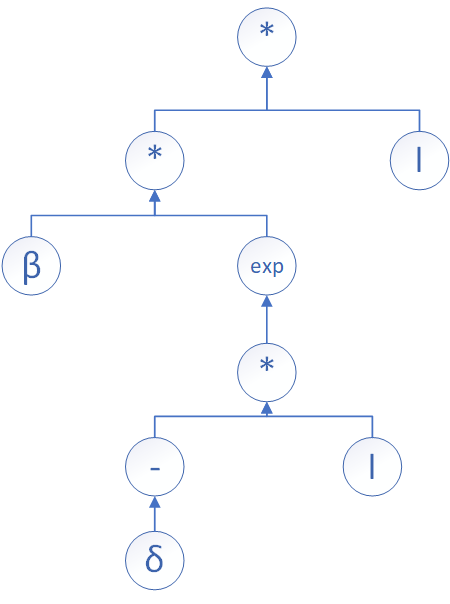
\includegraphics{./symbolictree.png}

The function can be discovered by using symbolic regression, where the
codes implemented in Julia are as following.

\section{IMPORTANT: Activate Julia environment
first}\label{important-activate-julia-environment-first-3}

\begin{Shaded}
\begin{Highlighting}[]
\ImportTok{using} \BuiltInTok{Pkg}
\BuiltInTok{Pkg}\NormalTok{.}\FunctionTok{activate}\NormalTok{(}\StringTok{"."}\NormalTok{)}
\end{Highlighting}
\end{Shaded}

\begin{Shaded}
\begin{Highlighting}[]
\CommentTok{\# Load packages}
\ImportTok{using} \BuiltInTok{SymbolicRegression}
\ImportTok{using} \BuiltInTok{SymbolicUtils}
\CommentTok{\# Generating test data}
\NormalTok{I }\OperatorTok{=} \FunctionTok{collect}\NormalTok{(}\FloatTok{0}\OperatorTok{:}\FloatTok{0.1}\OperatorTok{:}\FloatTok{10}\NormalTok{)}
\FunctionTok{f}\NormalTok{(x) }\OperatorTok{=} \FloatTok{0.2}\FunctionTok{exp}\NormalTok{(}\OperatorTok{{-}}\FloatTok{0.1}\OperatorTok{*}\NormalTok{x)}\OperatorTok{*}\NormalTok{x}
\NormalTok{Y }\OperatorTok{=} \FunctionTok{f}\NormalTok{.(I)}


\CommentTok{\# choosing operations}
\NormalTok{options }\OperatorTok{=}\NormalTok{ SymbolicRegression.}\FunctionTok{Options}\NormalTok{(}
\NormalTok{    binary\_operators}\OperatorTok{=}\NormalTok{(}\OperatorTok{+}\NormalTok{, }\OperatorTok{*}\NormalTok{, }\OperatorTok{{-}}\NormalTok{),}
\NormalTok{    unary\_operators}\OperatorTok{=}\NormalTok{(exp,),}
\NormalTok{    npopulations}\OperatorTok{=}\FloatTok{20}
\NormalTok{)}


\CommentTok{\# equations searching}
\NormalTok{hallOfFame }\OperatorTok{=} \FunctionTok{EquationSearch}\NormalTok{(I}\OperatorTok{\textquotesingle{}}\NormalTok{, Y, niterations}\OperatorTok{=}\FloatTok{150}\NormalTok{, options}\OperatorTok{=}\NormalTok{options, parallelism}\OperatorTok{=:}\NormalTok{multithreading}
\NormalTok{)}
\CommentTok{\# output}
\NormalTok{dominating }\OperatorTok{=} \FunctionTok{calculate\_pareto\_frontier}\NormalTok{(I, Y, hallOfFame, options)}
\NormalTok{eqn }\OperatorTok{=} \FunctionTok{node\_to\_symbolic}\NormalTok{(dominating[}\KeywordTok{end}\NormalTok{].tree, options)}
\end{Highlighting}
\end{Shaded}

\begin{verbatim}
(x1 * exp(-0.8866729615216796 - ((x1 - 5.823564614359717) * 0.10000000003526198))) * 0.27113961336456716
\end{verbatim}

\section{Project: predicting the peak
time}\label{project-predicting-the-peak-time}

Some immature ideas (may be wrong): - In Lectures 1\&2 note, we know
that
\[I(t_p)=I_0+S_0\left(1-\frac{1}{\mathcal{R}_0}-\frac{\ln\mathcal{R}_0}{\mathcal{R}_0}\right),\]
which implies the peak time \[t_p=f(\mathcal{R}_0).\]

Q: Can we use symbolic regression to search \(f\)?

\begin{itemize}
\tightlist
\item
  For real case data, you can learn
  \(\beta(t)=\mathrm{NeuralNetwork}(t)\) first \[
    \left\{
    \begin{aligned}
         & \frac{\mathrm{d}S}{\mathrm{dt}} = - \mathrm{NeuralNetwork}(t) S I,        \\
         & \frac{\mathrm{d}I}{\mathrm{dt}} = \mathrm{NeuralNetwork}(t) S I- \gamma I,
    \end{aligned}
    \right.
  \] then you get a new ODE. Solving this new ODE and setting
  \(\mathrm{NeuralNetwork}(t) S(t) I(t)- \gamma I(t)=0\), you can solve
  the peak time \(t_p\), and check whether \(t_p\) is minimum or maximum
  by checking the sign
  \[\frac{\mathrm{d}^2 I}{\mathrm{dt}^2}=(\mathrm{NeuralNetwork}(t) S I- \gamma I)'=(\mathrm{NeuralNetwork}(t)' S + \mathrm{NeuralNetwork}(t) S')I +(\mathrm{NeuralNetwork}(t) S - \gamma)I'.\]
\end{itemize}

Q: - How to solve this fixed point problem
\(\mathrm{NeuralNetwork}(t) S(t) I(t)- \gamma I(t)=0\)? - How to improve
the generalization (prediction ability) of the neural network embedded
in differential equations? - How to combine these two ideas?



\end{document}
